\section{Literature Review}

Magnetic coils have been employed as a simple and efficient torque production method for attitude and momentum control since the dawn of the space age \cite{silani2005magnetic}. Their performance is based on the interaction of the magnetic field generated by the coils and the earth’s magnetic field, and so provides a straightforward solution to the problem of creating torques on board a satellite \cite{silani2005magnetic, wertz2012spacecraft}. As a result, the torques that can be applied to the spacecraft for attitude control are confined to lie in the plane perpendicular to the magnetic field vector. In instance, 3 axis magnetic stabilization is only feasible if the orbit under consideration sees a variation in the magnetic field sufficient to ensure the spacecraft's stability \cite{lovera2001periodic}. Sidi \cite{sidi1997spacecraft} proposed a solution in which a magnetic coil is replaced with a reaction wheel in any of the body frame’s axes. Therefore the spacecraft becomes fully-actuated.


High angular velocity can be created during launch vehicle deployment or occur spontaneously in orbit owing to disturbance torques. Consequently, one important mission after the satellite gets launched into space is to detumble its angular velocity \cite{yadav2020investigation}. When the angular rate of a satellite in low Earth orbit (LEO) drops to 0.13 degree/s or below, it is considered detumbled \cite{andresen2005attitude}. Detumbling is a necessary procedure since it comes before any other operation on the satellite that requires some degree of attitude control. There are a variety of detumbling controllers available, and several of them have been tested in \cite{pignede2014detumbling} for a CubeSat. In terms of maneuver time, precision, control effort, robustness, and implementation. Controllers based on magnetometer feedback, gyroscope feedback, sun sensor feedback, and passive control are compared. The magnetometer feedback B-dot controller was determined to be the best and easiest to implement controller for a CubeSat.


There are other modes for the satellite to keep it pointing or aligned to specific axes as discussed in \cite{markley2014fundamentals}.
Some methods and approaches to the problem of Earth-pointing attitude control for a spacecraft using magnetic actuators are provided, which ensures virtually global closed loop stability of the desired relative attitude equilibrium for the spacecraft. As proposed by \cite{silani2005magnetic, lovera2006global} PD controller provides attitude regulation in the case of three controllers in the three axes. The nonlinear H-infinity state feedback attitude control method is designed for large spacecraft maneuvers and more convenient with control systems based on thrusters as discussed in \cite{jonsson2019simulations}.

Additionally, robust controllers have been developed to overcome inaccuracies in modeling and noise effects \cite{markley2014fundamentals}. Moreover, \cite{crassidis2000optimal} devised yet another robust control technique based on a nonlinear H-infinity control mechanism. This approach entails solving Hamilton-Jacobi-Isaacs inequalities, which effectively determine feedback gains for the whole state feedback control problem, allowing the spacecraft to be stabilized in the presence of uncertainties and disturbances. Variable structure control is robust to generic model parameter errors, but it comes at the expense of potentially high control activity.  Adaptive controllers update the model during operation based on measured performances \cite{markley2014fundamentals}. An adaptive scheme which estimates external torques by tracking a Lyapunov function has been developed by \cite{schaub2001adaptive}. This method has been shown to be very robust in the presence of spacecraft modeling errors and disturbances.

Controlling a satellite without full state feedback is a more difficult problem. Methods for estimating unavailable states using a filter algorithm and methods for developing control laws directly from output feedback are the two basic approaches used to solve this problem \cite{markley2014fundamentals}. 


\section{Detumbling}

\subsection{B-dot Controller}
The torque produced by magnetic torquers is given by
\begin{equation} \label{eqn:control_law}
    \mathbf{L} = \mathbf{m} \times \mathbf{B}
\end{equation}
where $\mathbf{m}$ is the torquer-generated commanded magnetic dipole moment and $\mathbf{B}$ is the local geomagnetic field in body-frame coordinates. The magnetometers' magnetic dipole moment is controlled to detumble the satellite from its arbitrary initial spinning by 
\begin{equation}
    \mathbf{m} = - \frac{k}{\norm{\mathbf{B}}} \mathbf{\dot{B}}
\end{equation}
where $k$ is a scalar gain \cite{markley2014fundamentals}. 
\subsection{Simulation Setup}
A MATLAB simulation framework with the configuration of the block diagram in figure \ref{fig:block} is created. An orbital propagator, an attitude propagator, a function to calculate attitude disturbance torques, and a magnetometer function are all part of this framework. It should be simple to change orbital, satellite, and hardware parameters. Each of the functions shown in figure \ref{fig:block} will be supplied along with this thesis.
\clearpage

\begin{figure}
    \centering
    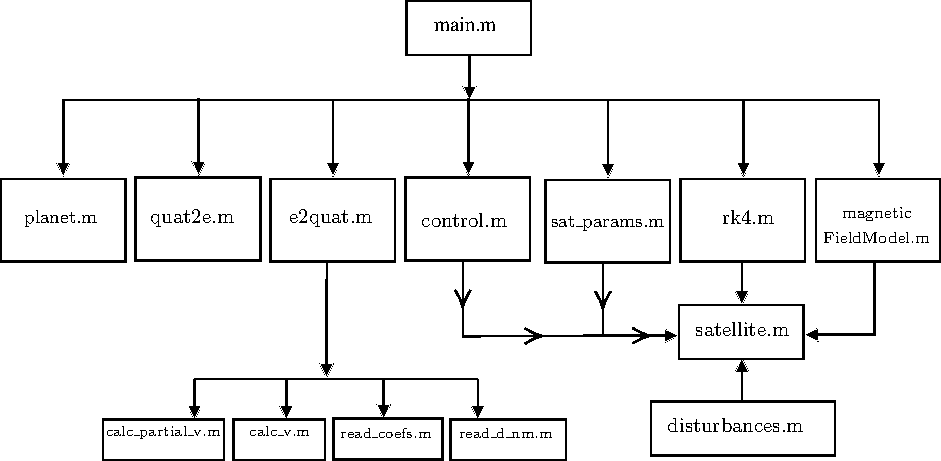
\includegraphics[width = \textwidth]{Figures/flow_chart.pdf}
    \caption{A block diagram of the simulation framework together with the detumbling controller.}
    \label{fig:block}
\end{figure}
The simulation in this section is carried out for the given parameters in table \ref{tab:parms}.
The satellite motion is simulated for orbits and the results obtained can be found in section \ref{sec:sim_res}.
\begin{table}[h]
    \centering
    \begin{tabular}{@{}cc@{}}
    \toprule 
     Parameter & Value \\
    \midrule 
     Semimajor Axis (Km) & 9122 \\
    Eccentricty & 0.1 \\
    Inclination (deg) & 120 \\
    Altitude (Km) & 450 \\
    $ I_{x}$ ($ Kg.m^{2}$) & 0.1 \\
    $ I_{y}$ ($ Kg.m^{2}$) & 0.2 \\
    $ Iz$ ($ Kg.m^{2}$) & 0.3 \\
    $ \omega_{x0}$ (deg) & 5 \\
    $ \omega_{y0}$ (deg) & 5 \\
    $ \omega_{z0}$ (deg) & 5 \\
     \bottomrule
    \end{tabular}
    \caption{Cube-sat simulation parameters}
    \label{tab:parms}
\end{table}
\clearpage


\subsection{Simulation Results} \label{sec:sim_res}
The b-dot control law in equation \ref{eqn:control_law} was simulated for a small satellite in low earth orbit for 3 orbits, the satellite and the orbit parameters are given in table \ref{tab:parms}. The initial angular rate is set to $\omega_0 = \begin{bmatrix} 5 & 5 & 5 \end{bmatrix}$ deg/sec. The controller gain is set to $k = 90 \times 10^3$. Figure \ref{fig:omega_cont} shows the response of $\boldsymbol{\omega}$ to the control torque, figure \ref{fig:omega_zoom} shows a zoom into the angular rate which entails that the controller managed to detumble the satellite to around $0.15$ deg/sec in 6000 sec. 
\begin{figure}[H]
    \centering
    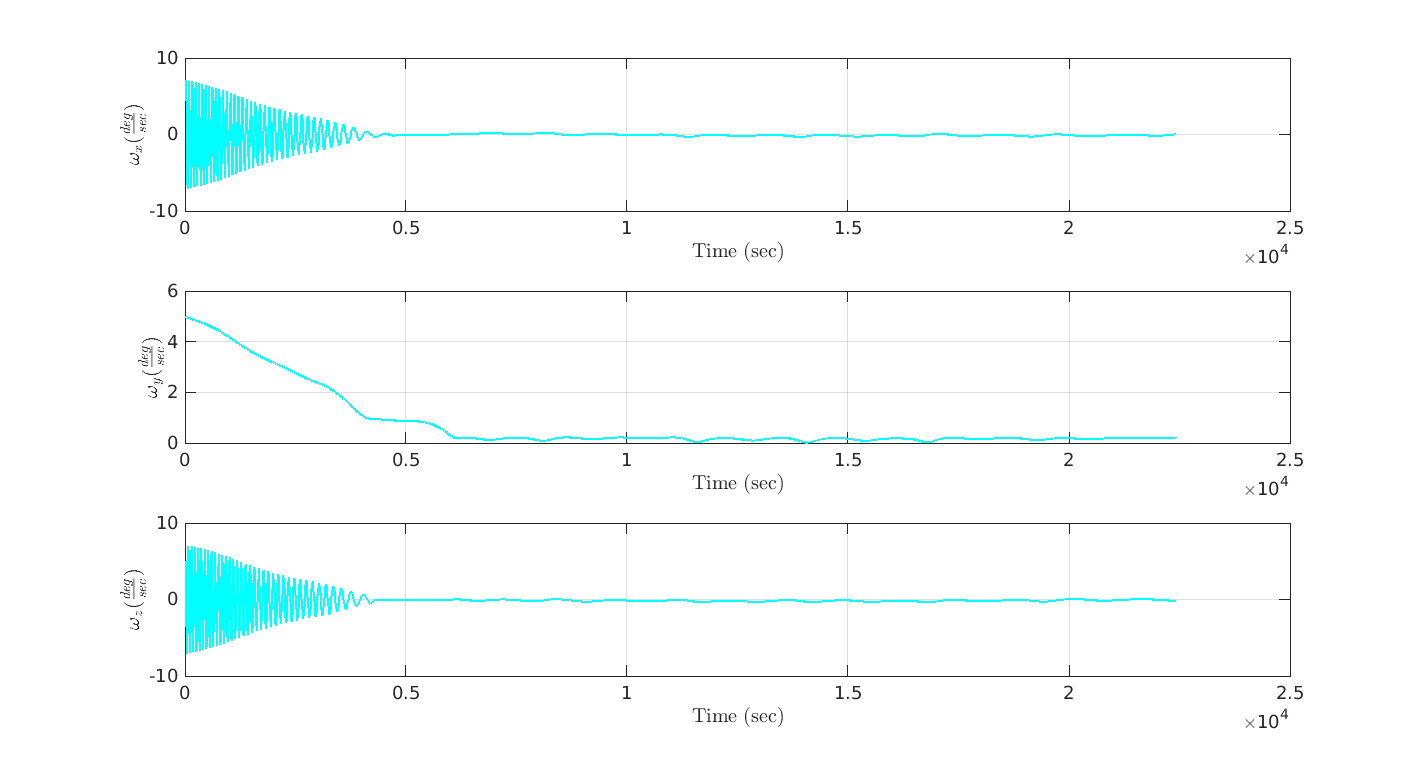
\includegraphics[width=0.8\textwidth]{Figures/omega_x_y_z.png}
    \caption{The controlled angular rate $\omega$ of the satellite for the case of detumbling}
    \label{fig:omega_cont}
\end{figure}
\begin{figure}[H]
    \centering
    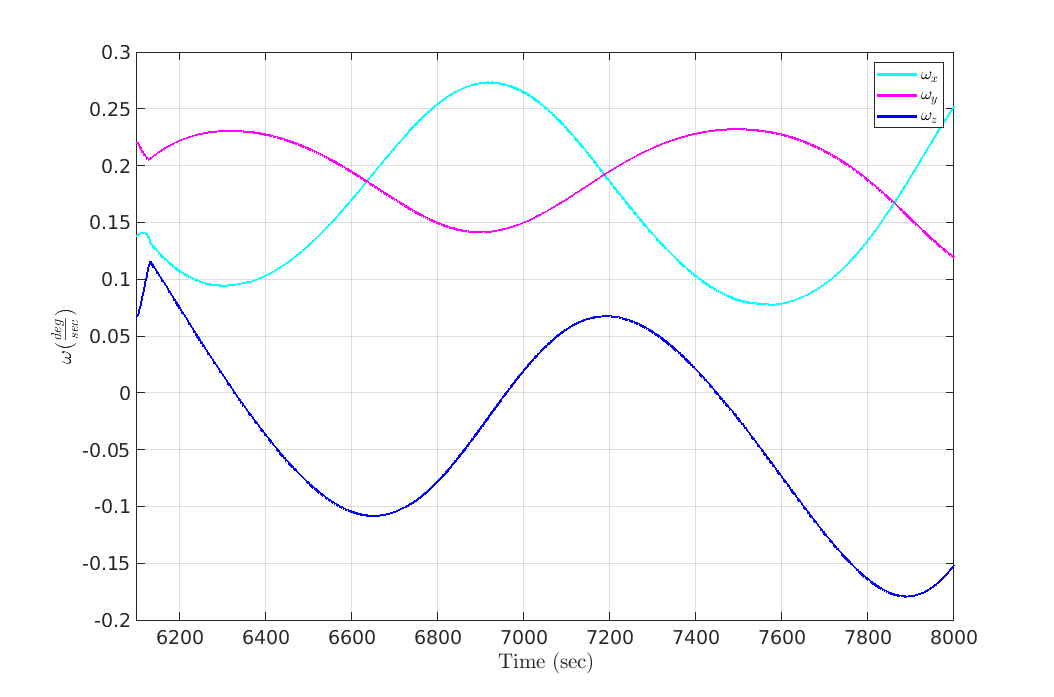
\includegraphics[width=0.8\textwidth]{Figures/zoom.png}
    \caption{Zoom into controlled angular rate $\omega$ of the satellite}
    \label{fig:omega_zoom}
\end{figure}
Figure \ref{fig:ptp_cont} shows the behaviour of the satellite described by Euler angles.
\begin{figure}[H]
    \centering
    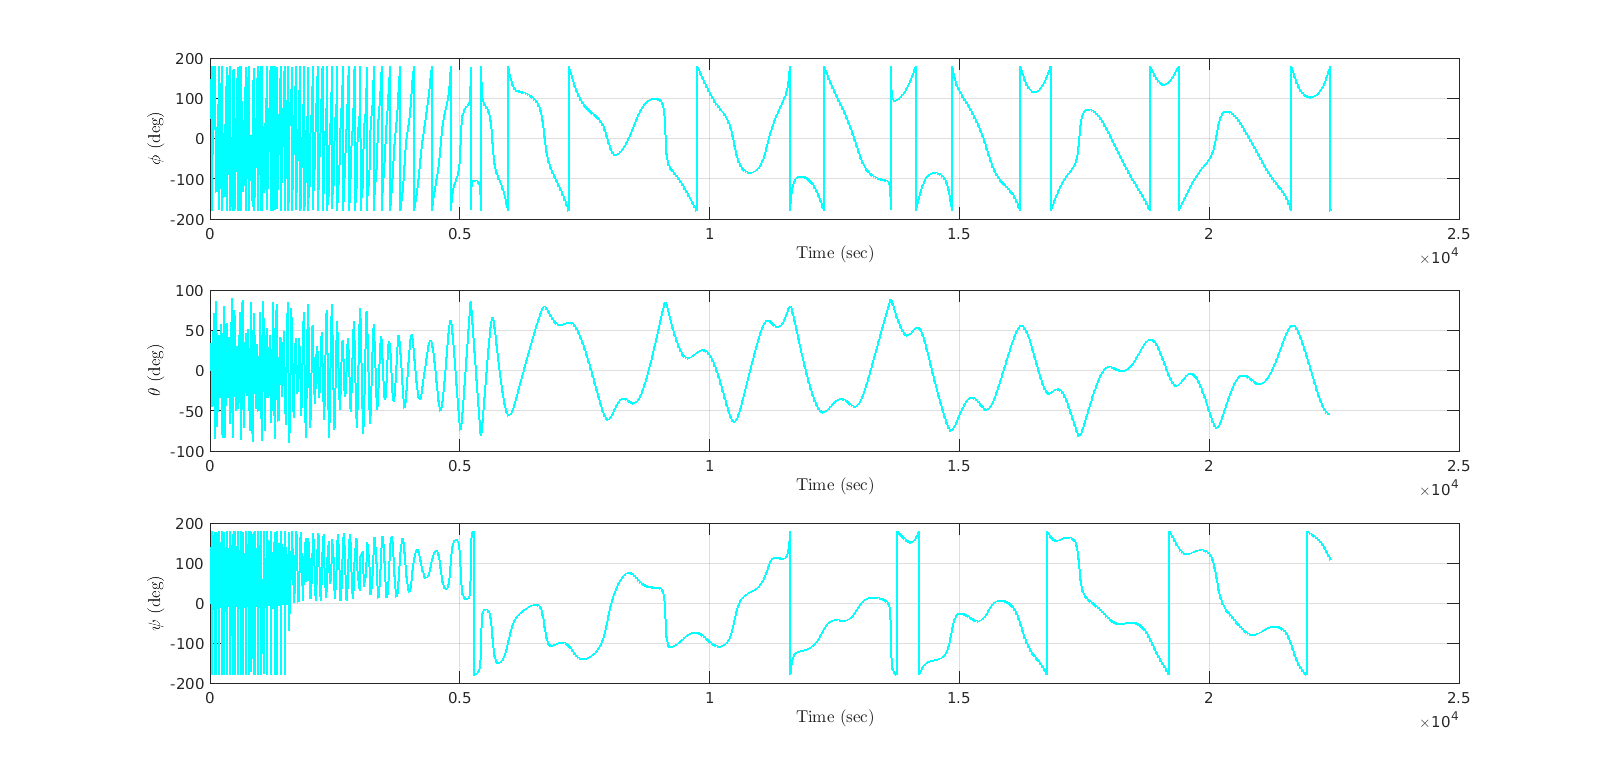
\includegraphics[width=0.8\textwidth]{Figures/ptp.png}
    \caption{The controlled Euler angels of the satellite for the case of detumbling}
    \label{fig:ptp_cont}
\end{figure}

\clearpage